\documentclass[ms,english]{stthesis}
\usepackage{lipsum}
\usepackage[color=green]{todonotes}
\usepackage{graphicx}
\usepackage{epigraph}
\usepackage{cite}
\usepackage[most]{tcolorbox}

\newcommand{\todor}[1]{\todo[color=green,inline,size=\small]{Reviewer: #1}}
\newcommand{\todoy}[1]{\todo[color=yellow,size=\small]{Oleksandr: #1}}

\definecolor{block-gray}{gray}{0.85}
\newtcolorbox{blockquote}{colback=block-gray,grow to right by=-1mm,grow to left by=-1mm,boxrule=0pt,boxsep=0pt,breakable}

\title{Compositional multi-objective parameter tuning}
\author{Oleksandr Husak}
\date{\today}
\birthday{16.04.1994}
\birthplace{Ukraine}
\supervisor{MSc. Dmytro Pukhkaiev \newline Dr.-Ing. Sebastian Götz}

\begin{document}
    \maketitle % This sets the title page
  
    \tableofcontents
  
    \section{Abstract}
    The multi-objective decision making is critical for an everyday task and also for engineering problems. Find perfect trade-off to enhance all criteria requires much experience or the availability of a significant amount of resources; that it is not feasible to achieve for an expensive problem such as engineering. The state-of-the-art approach is model-based or surrogate-based optimization that used approximation models of the real problem that is cheap to evaluation. These models are a simplified hypothesis of cause-effect relationships and replace high estimates with cheap approximations. In this thesis, we used surrogate models as wrappers on the real problem and applied \gls{moea} to detect  Pareto optimal decisions. 
    
    The general idea is combining and stacking several models that describe multiple objective sub-space independently and optimize it as a single surrogate hypothesis - surrogate compositional model. Combination of multiple models gave potential to approximate more complicated problems and stacking of valid surrogate hypothesis speed-up convergence. Accordingly, a better result is obtained at lower costs.
    We combine several possible surrogate variants and use those that pass validation. After recombination of valid single objective surrogates to a multi-objective surrogate hypothesis, several instances of \gls{moea}s provide several Pareto-front approximations. The modular structure of implementation allows us to avoid static sampling plan, use self-adaptable models with customizable portfolio. In numerous case studies, our methodology finds comparable solutions to standard NSGA2 using considerably fewer evaluations. The developed approach is recommended for parameter tuning of expensive black-box functions.
    \chapter{Introduction}\label{sec:intro}

\begin{blockquote}
\paragraph{Intent:} A short version of thesis and a description of done work. Challenges and Problems.

    \begin{description}
        \item[1. Motivation] Surrogate model for multi-objective expensive black-box problem $\rightarrow$ Research gap: Portfolio/Compositional system/Sampling plan. Definition and motivation of the goal. Goal: MO solution $\rightarrow$ Problem: Expensive black-box $\rightarrow$ Solution: Answer research questions
        \item[2. Objectives of work] ?
        \item[3. Research Questions] Question from research gap. The answer to this questions is the purpose of the thesis
        \item[4. Results overview] A short overview of done work
    \end{description}
\end{blockquote}

% --------------------------------------------------------------------------------------------
% ------------------------------------------------     Motivation      
% --------------------------------------------------------------------------------------------
\section{Motivation}

    In traditional manual parameter tuning, engineers put the effort in searching the optimal objectives guided by experience and intuition. Regardless, many of these optimization problems have a huge search space that could be handled only with automatic tools. This kind of software could extrapolate and highlight the most perspective parameters from infinite space, but at the same time, struggle in multi-criteria decisions that are critical for engineering problems. For examples: architecture design, test generating, tuning machine-learning algorithms or experiment plan could be stated as multi-objective problems. To understand the space of possible solution, they are represented on the Pareto frontier; i.e. the subset os solutions that could be not improved in some objectives without degrading in another.
    Multi-objective algorithms or single-objective with scalarization allows to find out some Pareto optimal points. Still, they require a massive amount of evaluations that are not appropriate for an expensive problem. A common approach to reducing the final cost of the optimization algorithm is to replace some expensive estimations with cheap ones with the help of surrogate models. The conventional algorithms to extrapolate available results are Bayesian Regression model(Kriging), Neural Network, SVR or combinations of Tree regressions(Decision) estimators. Regardless, almost all optimizations use static models or aggregation several instances of one model type. These approaches lack variability and cannot be finely tuned.

    This thesis introduces a modular structure for multi-objective parameter tuning that allows to use of compositional diverse surrogate models and apply various optimization techniques. This goal was accomplished by a surrogate portfolio, stepwise validation and a combination of final decisions. The evaluation on various problems showed excellent results and superiority over analogues methodologies. Composition of surrogate models can be used to improve the applicability of model-based optimization to a verity of problems such as parameter tuning.




    % Surrogate model or models based optimization is a common approach for a deal with expensive black-box function, but as far as the author is aware, there is no published research where the influence of heterogeneous portfolio of surrogate models was studied. The main target problem is an expensive multi-objective problem but the developed approach is also suitable for expensive single-objective optimization.
    % As black-box, we can not say what type of surface does the problem have. That is why it should be customized in the optimization process. The goal is to determine if the variability in extrapolation worth it. Introduce new surrogate-design-criteria for multi-objective hyperparameter optimization software.

    % It also provides backward compatibility for a single-objective problem. This optimization approach can significantly reduce expensive evaluations counts but torment from problems such as sampling size, type of surface and optimization techniques. We developed and adopted new technic in MBO such as portfolio surrogates, compositional model and surrogate validation. 

    % Multi-objective optimisation is an established parameter tuning technique. It is especially suited to solve complex, multidisciplinary design problems with an accent on system design.

    % When we talk about several objectives, the intention is to find good compromises rather than a single solution as in global optimization.
    % Since the solution for multi-objective optimization problems gives the appearance to a set of Pareto-optimal points, evolutionary optimization algorithms are ideal for handling multi-objective optimization problems.

    % General optimization methods could be classified into derivative and non-derivative methods. In this thesis focuses on non-derivative methods, as they are more suitable for parameter tuning. Therefore, they are also known as black-box methods and do not require any derivatives of the objective function to calculate the optimum.  Other benefits of these methods are that they are more likely to find a global optimum. 


% --------------------------------------------------------------------------------------------
% ------------------------------------------------     Objectives      
\section{Objectives}
        Develop strategies that can decompose the surrogate model into several single-objective models, and enhance bast practices in single-objective parameter tuning.

    % --------------------------------------------------------------------------------------------
    % ------------------------------------------------     Research Questions      
    \section{Research Questions}
    The goal of this thesis is to provide a mechanism of a fined-grained models composition that allows making a multi-objective decision as software product-line for parameter tuning. The criterion for reaching the goal is to reduce the number of objective evaluations while keeping the optimal quality of a decision.

    \begin{description}
        \item[RQ1:\label{RQ1}] Heterogeneous compositional surrogate models for multiobjective optimization
        \begin{itemize}
            \item[RQ1.1:\label{RQ1.1}] Scalable surrogate-based optimization
        \end{itemize}
        \item[RQ2:\label{RQ2}] Domain independent sampling strategies
    \end{description}

% --------------------------------------------------------------------------------------------
% ------------------------------------------------     Overview
\section{Results overview}
    In numerous test problems, the portfolio with compositional-surrogates finds comparable solutions to standard MOEA (NSGA-II, MOEAD, MACO, NSPSO) doing considerably fewer evaluations (500 vs 10000). Dynamic sampling accelerates the start of the optimization process and prevents wasting resources. The surrogate portfolio allows adapting the optimization process to concrete domain problem and the number of available samples. 

% \section{Solution}

% \section{Organization of the Thesis}

    \chapter{Foundation}

    \begin{blockquote}
        \paragraph{Intent:} General background information needed to follow the terms and methods used in this thesis.
        
        Structure:
        \begin{description}
            \item[1. Parameter tuning] Parameter tuning of a black-box
                \begin{enumerate}
                    \item $f(Parameter) = Objective$ 
                    \item Goal is optimize $f$
                    \item Problem: Optimization of multiple objectives
                \end{enumerate}
            \item[2. Multi-objective optimization] General definition. Pareto front and None-dominated solution
                \begin{enumerate}
                    \item What is a multi-objective solution?
                    \item How to compare solutions? $\rightarrow$ Types of metrics
                    \item How to solve? $\rightarrow$ Scalarizing, MOEA, Random
                    \item Problem: Reduce evaluations $\rightarrow$ Surrogate optimization, MBMO
                \end{enumerate}
            \item[3. Surrogate optimization] Approach for reducing evaluation count
                \begin{enumerate}
                    \item Intro. Cons and Pons
                    \item Types of a surrogate model in a MO-problem (Model of scalarization, MO-model, Replicated MO-model, Compositional MO-model). Taxonomy
                    \item Surrogate assistance for MO parameter tuning $\rightarrow$ Reusable/scalable components for optimization $\rightarrow$ Problem: Scalability of a surrogate model. [RQ2 \ref{RQ2}]                   
                    \item Surrogate model is domain-specific $\rightarrow$ Analyze multiple surrogates $\rightarrow$ Surrogate portfolio [RQ1 \ref{RQ1}]
                    \item Sampling plan. Build a surrogate model. Quality of prediction depends on the accuracy of a surrogate model  $\rightarrow$ Accuracy depends on a sample size $\rightarrow$ Sample size depends on surface type $\rightarrow$ Problem: Sample size is static. [RQ3 \ref{RQ3}]
                \end{enumerate}
            \item[4. Scope of work] Starting point of thesis
                \begin{enumerate}
                    \item Problem: Expensive black-box with multiple objectives
                    \item Constraint: Evaluation budget
                    \item Goal: Set of MO solutions closed to Pareto-front $\rightarrow$ 1.$Max$ Hypervolume, 2.$Min$ Points-Space, 3.$Max$ \% of None-Dominated points 
                    \item Solution approach: Surrogate model(s) with MOEA
                \end{enumerate}
        \end{description}
    \end{blockquote}

    \paragraph{Intro}
    In this chapter present general background information needed to follow the terms and methods used in this thesis. What is parameter tuning? Why multi-objective is important? Why we can't use the standard multi-objective approach in real-life problem/parameter tuning task, and why model-based or surrogate optimization is the best solution?

    In common old-fashioned software design, engineers carefully convert overall models into domain-specific tools. In this approach, designers codify the current understanding of the problem into the parameters. 

    % --------------------------------------------------------------------------------------------
    % ------------------------------------------------        Parameter tuning
    % --------------------------------------------------------------------------------------------
    \section{Parameter tuning}

        Given recent advances in computing hardware, software analysts either validate engineer models or find optimal configuration by using parameter tuning tools to explore thousands to millions of inputs for their systems. 

        In this article assume that parameter tuning is a subset problem of general, global optimizations. It's also mean that we consider some fitness function $f$ that converts the parameter vector to output objectives.  Note that the term "real evaluation" or "black-box evaluation" as a synonym for the fitness function $f$. 
        
        The goal of parameter tuning as an optimization task lay on fast iterative search with improvements in each objective dimension. The term "fast" means that the convergence to global optimum is achieved with the least real evaluations and shorter time frame.

        We consider fitness function $f$ as black-box with parameter and objective space. Parameter space has structure and could consist from continues and categorical dimensions. Sometimes, some combinations of parameter settings are forbidden. Each point from parameter space lead to some point in objective space. Configurations often yield qualitatively different behavior.
        Objective space also could be described as usual objectives as accuracy, runtime, latency, performance, error rate, energy and so on. On each objective should gain the best possible value and rich system tradeoff.

        Optimization technics:
        \begin{itemize}
            \item Grid search vs Random search
            \item Heuristics and Metaheuristic. (Simulated annealing, Evolutionary algorithm..) These methods aim at generating approximately optimal solutions in a single run. Also could operate with sets of solutions being outcomes of multiple objectives.
            \item Sequential design (Bayesian optimization, Evolutionary algorithm..) Bayesian methods differ from random or grid search in that they use past evaluation results to extrapolate and choose the next values to evaluate. Limit expensive evaluations of the objective function by choosing the next input values based on those that have done well in the past.
        \end{itemize}

        Optimization cost of black-box:
        \begin{itemize}
            \item Evaluation may be very expensive
            \item Sampling budget is unknown
            \item Possibly noisy objectives
            \item Feasibility constraints
            \item Multi-objectivity
        \end{itemize}

        Ideally, we want a method that can explore the search space while also limiting evaluations of hyperparameter choices. 
        The single criterion in parameter tuning may not be sufficient to correctly characterize the behaviour of the configuration space that is why multiple criteria have to be considered.
        One way to clarify the task of understanding the space of possible solutions is to focus on the non-dominated frontier or Pareto-front, the subset of solutions that are not worse than any other but better on at least one goal. The difficulty here is that even the Pareto frontier can be too large to understand. 
    

    % --------------------------------------------------------------------------------------------
    % ------------------------------------------------        Multi-objective       -------------
    % --------------------------------------------------------------------------------------------
    \section{Multi-objective optimization}

        Parameter tuning is present in our daily life and comes in a variety of states. The goal is the rich best possible objective by correctly choosing the system parameters. 
        Common of optimization problems requires the simultaneous optimization of multiple, usually contradictory, objectives. These type of problems are termed as multiobjective optimization problems. The solution to such problems is a family of points, that placing on a Pareto front. Knowledge of the Pareto front allows visualizing appropriate decisions in terms of performance for each objective.

        "Multi-objective optimization(MOO) deals with such conflicting objectives. It provides a
        mathematical framework to arrive at optimal design state which accommodates the various criteria demanded by
        the application. The process of optimizing systematically and simultaneously a collection of objective functions
        are called multi-objective optimization (MOO) \cite{odugod2013}".

        For a multi-objective problem, we consider "solution" as points from parameter space that lead to non-dominated results in objective space. This set of points approximate real Pareto-front. Improving "solution" means that sets of points coincide better with real Pareto-front.

    % ------------------------------------------------        Metrics       -------------
        \subsection{Metrics for multi-objective solution}

        In single-objective minimization, the quality of a given solution is trivial to quantify:
        the smaller the objective function value, the better. However, evaluating the quality of an approximation of a Pareto set is non trivial.
        The question is important for the comparison of algorithms or prediction next configuration.

        According to \cite{ZitzlerDT00}, a Pareto front approximation should satisfy the following:
        \begin{itemize}
            \item The distance between the Pareto front and its approximation should be minimized.
            \item A heigh distribution of the non-dominated points is desirable.
            \item The range of the approximated front should be maximized, i.e., for each objective, a wide range of values should be covered by the non-dominated points.
        \end{itemize}

        Metrics for performance indicators partitioned into four groups according to their properties \cite{Audet2018PerformanceII}: 
        \begin{itemize}
            \item cardinality
            \item convergence
            \item distribution
            \item spread
        \end{itemize}

        Base on the right metrics general multi-objective algorithm keep making progress toward the Pareto front in the objective function space.
        The goal of optimizing a multi-objective problem is to obtain an approximation solution set to the reference Pareto front, including the following subgoals:
        \begin{itemize}
            \item All solution set are as close as possible to the Pareto front
            \item All solution set are as diverse as possible in the objective space
            \item Evaluate as few solution as possible
        \end{itemize}
        Straightforward applying of the simple coefficient of determination (R2) is the wrong indicator of success. Evaluations of different sets of Pareto optimal points is multi-objective task.
        The necessary objectives follow for improving solutions:
        \begin{itemize}
            \item Keep hypervolume low. Reference point is 0 for all objectives.
            \item Maximize sparsity of points. Average distance. Crowding Distance. Spacing metrics.
            \item Maximize non-dominant decisions in the total population
        \end{itemize}

        Also distribution and spread indicators is consider in this work. According to \cite{CustodioMVV11}, “the spread metrics try to measure the extents of the spread achieved in a computed Pareto front approximation”. They are not useful to evaluate the convergence of an algorithm, or at comparing algorithms. They only make sense when the Pareto set is composed of several solutions.

        For multi-objective optimization (MOO), an algorithm should provide a set of solutions that realize the optimal trade-offs between the considered optimization objectives, i.e., Pareto set. Therefore, the performance comparison of MOO algorithms is based on their Pareto sets. In this study, three popular metrics are used to quantify the performance of the algorithms. 
        \begin{itemize}
            \item Hypervolume (HV)\cite{Zitzler2000ComparisonOM}. 
            This metric represents the volume of the objective space that is covered by the individuals of a non-dominated solutions set (solutions that belong to a Pareto front). The volume is delimited by two points: one point that is called the anti-optimal point (A) that is defined as the worst solution inside the objective space, and a second optimal point (pseudo-optimal) that is calculated by the proposed solution method. 
            Determining the hypervolume indicator is a computationally expensive task. Even in case of a reasonably small dimension and low number of points (e.g. 100 points in 10 dimensions), 
            there are currently no known algorithms that can yield the results fast enough for use in most multiple-objective optimizers
            \item Non-dominated Ratio (NDR). This metric employs the non-dominated count of a solution set divided by the total size of solution set. Higher values are preferred to lower ones.
            \item Spacing \cite{Schott1995FaultTD}. Describe the distribution of Pareto points. Fewer space metrics means better coverage of objectives values range.
            
        \end{itemize}

    % ------------------------------------------------        Solving methods       -------------
        \subsection{Solving methods}
        How to search for an optimal solution to the multi-objective optimization problem?
        
            % ----------------      Scalarizing       
            \subsubsection{Scalarizing}
                Scalarizing approach is built on the traditional techniques to creating an alternative problem with a single,
                composite objective function. Single objective optimization techniques are then applied to this composite function to obtain a single optimal solution.
                The weighted-sum methods it's a well known type of scalarizing technic is applied to simplify a multiobjective problem. Concatenate the objectives into one criterion by using magic weighted sum factors. 
                The merged objective is used to evaluate and define the optimal solution.
                Weighted sum methods have difficulties in selecting proper weight especially when there is no connected a priori knowledge among objectives.
                Furthermore, Uniform distribution points in parameters space don't generate uniform distribution points on objective space. This means that we can't approximate Pareto-front completely even with multiple optimization rounds.
                Some scalarizing technics try to improve exploration of parameter space by assigning more "intelligence" aggregation to the objectives. Such solutions may be fragile. They change dramatically if we modify algorithm parameters.

                Moreover, the weighting method can not provide a solution among underparts of the Pareto surface due to “duality gap” for not convex cases. Even for convex cases, for example, in linear cases, even if we want to get a point in the middle of a line segment between two points, we hardly get a peak of Pareto surface, as long as the well-known simplex method is used. This implies that depending on the structure of the problem, the linearly weighted sum can not necessarily provide a solution as DM desires. \cite{Nakayama05}

            % --------------------      MOEA
            \subsubsection{Multi-Objective Evolutionary Algorithms}

                Generating the Pareto set can be computationally expensive and is often infeasible because the complexity of the underlying volume limits exact techniques from being applicable. For this reason, a number of stochastic search strategies such as evolutionary algorithms, tabu search, simulated annealing, and ant colony optimization have been developed: they usually do not guarantee to identify optimal trade-offs but try to find a good approximation, i.e., a set of solutions whose objective vectors are (hopefully) not too far away from the optimal objective vectors \cite{EmmerichD18}.

                The evolutionary algorithm (EA) form a class of heuristic search methods that simulate the process of natural evolution.
                Using simplifications, this EA is subsequently determined by the two basic principles: selection and variation.
                While selection imitates the competition for reproduction and resources among living beings, the other principle, variation, imitates the natural ability to create ”new” living beings through recombination and mutation. Evolutionary algorithm possesses several characteristics that are desirable for problems including multiple conflicting objectives, and large and complicated search spaces. However, EA still need many evaluations of the "black box" system to solve a common multi-objective problem. This is further complicated by the fact that many such problems are very expensive. Consolidated, this makes EAs unfeasible for costly and Multy-objective problem.
                A good solution is the integration of the surrogate model which extrapolate and approximate the fitness landscape from samples. Multi-objective Evolutionary Algorithms (MOEAs) use this surrogate model as a target for optimization. Assumed that solution from surrogate nearby to a global optimum.
                The goal of this thesis is to understand if the performance of MOEAs approach can be improved by using compositional surrogates. The key idea of compositional surrogates is the splitting objective space to multiple surrogates that extrapolate it independently.Combination of multiple hypotheses should give them the potential to approximate more complicated problems. This approach avoids the idea of a single surrogate model, preferring instead to use the composition hypothesis to split out the terrain of objective space.

                The multiple surrogates are analysed on objectives with various complexity, beside the simple and complicated unimodal structure. Generating a cloud of candidates is computationally expensive.

                Evolutionary optimizers explore populations of candidate solutions in each generation, some mutator can make changes to the current population. A select operator then picks the best mutants which are then combined in some way to become generation i+1. 
                This century, there has been much new work on multi-objective evolutionary algorithms with two or three objectives 
                (as well as many-objective optimization, with many more objectives). Multi-objective Evolutionary Algorithms (MOEAs) are popular tools to solve optimization problems, because of their applicability to complex fitness landscapes and solid performance on problems with large design spaces. While other methods also exist, in this thesis we will focus on improving approaches with Evolutionary Algorithms for the Multy-objective optimizations.
                This search-based software engineering is a rapidly expanding area of research and a full survey of that work is 
                beyond the scope of this thesis.

        % ------------------------------------------------        Conclusion       -------------
        \paragraph{Conclusion}
            Motivation for Surrogates

            For optimization expensive black-box:
            \begin{itemize}
                \item Scalable algorithms that convert multi-objective to single objective problem produce solution that not accurate enough(Scalarizing). Also this approach suitable for a limited type of problem. Also, there are a lot important parameters that significant influence on algorithm performance.
                \item Genetic algorithms. This approach is costly to perform and not appropriate for expensive problems.
            \end{itemize}
            Optimization gap in obtaining high quality, multi/single-obj solutions in expensive to evaluate experiments.
            Experiments as a black box, derivative-free. Reference to surrogate optimization.


    % --------------------------------------------------------------------------------------------
    % ------------------------------------------        Surrogate optimization       -------------
    % --------------------------------------------------------------------------------------------
    \section{Surrogate optimization} 

        The potential for applying surrogate is laid in the fast evaluation of the surrogate model. This advantage should outperform disadvantage in time required to build this surrogate model. In classical model-based optimization is used single surrogate-model that provide a hypothesis on the relation between parameter and objective space. There is a lot type of models that can do it but out and away fewer models that can manage multidimensionality objective space. The perspective way to create multi-objective surrogate is stacking multiple simple models into one that describes complex objective space. Notwithstanding that those models could be completely different and build in parallel, they still related because fitted on intersection features.
        Splitting optimization problem to multiple stages improves the reusability of code and makes approach scalable. Nevertheless, we can switch from single-obj to multi obj and change optimization technic on the fly.


        \begin{figure}
            \centering
            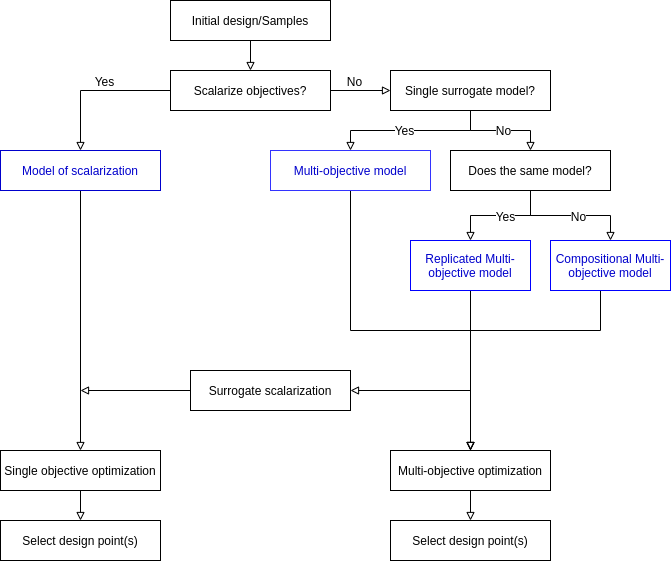
\includegraphics[width=\textwidth]{content/images/mbmo.png}
            \caption[Generalized MBMO algorithm]{Generalized MBMO algorithm}
            \label{fig:generalMBMO}
        \end{figure}


        A surrogate model is either selected randomly or due to its popularity in the area with which the problem is associated.  However, there are still some open challenges related to the ensemble of meta- models such as what should be the criterion for choosing different metamodels or how different metamodels can be used simultaneously? In addition, there are no guidelines for using different models for different objective functions \cite{SoftSurvey}.

        \cite{EngSurMod} 

        To dealing with expensive optimization problem more quickly, we can use surrogate models in the optimization process to approximate the objective functions of the problem. Approximation of solution is faster than the whole optimization process can be accelerated. Nevertheless, the extra time needed to build and update the surrogate models during the optimization process. 
        In the case of pre-selecting the promising individuals, the surrogate model is used to find the likely or drop the low-quality individuals even before they are exactly evaluated, thus reducing the number of exact evaluations.

        In the literature, the term surrogate or model-based optimization is used where, during the optimization processes, some solutions are not evaluated with the original objective function, but are approximated using a model of this function. Different approximation methods are used to build surrogate models. For single and multiobjective optimization similar methods are used. 
        These techniques typically return only one approximated value, which is why in multiobjective problems several models have to be used, so that each model approximates one objective. Some of the most commonly used methods are the Response Surface Method \cite{ResponseSurface}, Radial Basis Function \cite{Rasmussen2004}, Neural Network, Kriging \cite{Woodard00} and Gaussian Process Modeling \cite{RasmussenN10, RasmussenW06}.

        General classification \cite{MlakarPTF15}:
        Within surrogate-model-based optimization algorithms, a mechanism is needed to find a balance between the exact and approximate evaluations. In evolutionary algorithms, this mechanism is called evolution control \cite{Jin05} and can be either fixed or adaptive. In fixed evolution control the number of exact function evaluations that will be performed during the optimization is known in advance. Fixed evolution control can be further divided into generation-based control, where in some generations all solutions are approximated and in the others, they are exactly evaluated \cite{DebN07}, and individual based control, where in every generation some (usually the best) solutions are exactly evaluated and others approximated \cite{Grierson1993}. In adaptive evolution control, the number of exactly evaluated solutions is not known in advance but depends on the accuracy of the model for the given problem. Adaptive evolution control can be used in one of two ways: as a part of a memetic search or to pre-select the promising individuals which are then exactly evaluated \cite{PilatN12}.

        Surrogate used to expedite search for global optimum. Global accuracy of surrogate
        not a priority. Surrogate model is cheaper to evaluate than the objective.

        Bayesian optimization (BO) methods often rely on the assumption that the objective function is well-behaved, but in practice, the objective functions are seldom well-behaved even if noise-free observations can be collected. In \cite{bodin2019modulating} propose robust surrogate models to address the issue by focusing on the well- behaved structure informative for search while ignoring detrimental structure that is challenging to model data efficiently.

        % -------------------------------------------------------------------------------------------------
        % ------------------------------------------------        MO in Parameter tuning       -------------
        \subsubsection{Multi-objective parameter tuning}
        
            % -------------------       Surrogate-model in MOEA       
            \paragraph{Surrogate-model-based MOEA}
            In \cite{KrallMD15} proposed approaches that apply kind of surrogate assistant to evaluations and ranging new population. It allows detecting the most informative examples in population and evaluates them. 
            Identifies and evaluates just those most informative examples at the end done fewer evaluations of the real system. Another way to explore solutions is to apply some heuristic to decompose the total space into many smaller problems, and then use a simpler optimizer for each region. 

            Surrogates are also used to rank and filter out offspring according to Pareto-related indicators like the hypervolume \cite{EmmerichGN06}, or a weighted sum of the objectives \cite{TaboadaBCW07}. The problem with the methods that use hypervolume as a way of finding promising solutions is the calculation time needed to calculate the hypervolume, especially on many objectives. Another possibility is described in \cite{Li2009}, where the authors present an algorithm that calculates only non-dominated solutions or solutions that can, because of variance, become non-dominated. 
            
            GP-DEMO \cite{MlakarPTF15} The algorithm is based on the newly defined relations for comparing solutions under uncertainty. These relations minimize the possibility of wrongly performed comparisons of solutions due to inaccurate 
            surrogate model approximations. Using this confidence interval, we define new dominance relations that take into account 
            this uncertainty and propose a new concept for comparing solutions under uncertainty that requires exact evaluations 
            only in cases where more certainty is needed.


            % ------------------        Surrogate-model with MOEA       
            \paragraph{Surrogate with MOEA}
            Kind of extending the search stage of MOEA with surrogate to simulate evaluation of population. It transform the problem of searching a new better population to improving general hypothesis of how and where Pareto set presented.  

            In surrogate-model-based multiobjective optimization, approximated values are often mistakenly used in the solution comparison. As a consequence, exactly evaluated good solutions can be discarded from the population because they appear to be dominated by the inaccurate and over-optimistic approximations. This can slow the optimization process or even prevent the algorithm from finding the best solutions \cite{MlakarPTF15}. 
            
            % ------------------        Compositional architecture       
            \paragraph{Compositional architecture}
            We could describe compositional-based surrogate optimization as compound grey-box system whit a lot of open research areas where surrogate should improve, managing portfolio, compare of predictions Pareto fronts. 
            As a developer, you can be focused on a specific problem and don't know how to implement other components. This is one of the main advantages of the described approach.
    
            \paragraph{Compositional surrogates}
            Can the same single-objective models be equally applied to various types of problems in multi-/single-objective optimization?
            When there is no correlation between the objectives, a very simple way to solve this kind of problem is to build independent models, i.e. one for each objective, and then to use those models to simultaneously extrapolate possible solutions with MOEA. Nevertheless, the output values correlated, but an often naive way to build multiple models that able to extrapolate complex objective space is often given good results.  
    
            Later research generalized this approach. MOEA/D (multiobjective evolutionary algorithm based on decomposition \cite{ZhangL07}) is a generic framework that decomposes a multi-objective optimization problem into many smaller single problems, then applies a second optimizer to each smaller subproblem, simultaneously.
    
            With multiple models, their flaws can combine, as well as the time required to build the models. In memetic algorithms, especially if the surrogate model is not very accurate, a local optimum can be found instead of the global optimum. But in terms of parameter tuning, this point should be better than a predefined sampling plan. Evaluation of this prediction improve surrogate model quality in the near-optimal area and improve prediction in the next round.
            For example, OEGADO \cite{ChafekarSRX05} creates a surrogate model for each of the objectives. The best solutions in every objective get also approximated on other objectives, which helps with finding trade-off individuals. The best individuals are then exactly evaluated and used to update the models.
        

        % --------------------------------------------------------------------------------------------
        % ------------------------------------------------     Domain-specific Surrogate model      
        \subsection{Domain-specific problem}
        With gain to find the best solution with less effort surrogate models is domain-specific. It's mean that from two surrogate models in two different problems the best surrogate is changing. It could interpreter as Non-free lunch theorem in model-based optimization. If we extend this argument then the same optimization problem in different parameter tuning iteration could be interpreted as another optimization problem. This means that to reduce effort and increase the convergence of an algorithm we should change the surrogate model depend on how much samples do we have. As one would expect, no approximation method is universal.
        This leads us to use a portfolio with surrogate models. As a negative consequence, the model fitting additional introduces an additional overhead into the optimization.


        % --------------------------------------------------------------------------------------------
        % ------------------------------------------------     Build surrogate model     
        \subsection{Build the surrogate model(s). Sampling plan}



        % --------------------------------------------------------------------------------------------
        % -------------------------------------------------------        Discussion       ------------
        \paragraph{Discussion}
        Example of each type of optimization. Justification solution.
        Conclusion: Design gap in optimization/parameter tuning. 
        Need to indicate optimization workflow for expensive process/experiments. 
        The argument(s) why we need a new architecture. Reference to composition architecture.

        Surrogate based optimization has proven effective in many aspects of engineering and in applications where data is "expensive", or difficult, to evaluate.

    % --------------------------------------------------------------------------------------------
    % ------------------------------      Compositional Surrogate optimization       -------------
    % --------------------------------------------------------------------------------------------


    \section{Scope of work}
        \todo{make some nice tree-diagram}

        Describe and implement workflow for multi-objective parameter tuning of the derivative-free, black-box system. Parameter estimation is costly. The proposed solutions are also suitable for single-criteria optimization. Problem Setting.

        Goal:
        \begin{enumerate}
            \item Globally optimize an objective function(s) that is expensive to evaluate. Single/Multi-objective parameter tuning
            \item Simultaneously optimization scalable objectives
            \item Components reuse. Extensibility with other frameworks
        \end{enumerate}

        Problem:
        \begin{enumerate}
            \item A large number of the target black-box evaluations
            \item Interfaces not unify
            \item Code duplication
        \end{enumerate}

        Solution:
        \begin{enumerate}
            \item Component-Based Architecture
            \item Compositional-based surrogate optimization with MOEA
        \end{enumerate}

    \chapter{Concept}

    \paragraph{Into}
    \begin{enumerate}
        \item Classification approaches with surrogate model
        \item Define problems that related with surrogates model
        \item Ideas on how to solve it
        \item Discussion
    \end{enumerate}

    In this section general applicability of surrogate model presented. With different applicability use cases, there are some obstacles occurred that have a place to be in all circumstances.

    General problem trade-off is producing the best possible multi-objective solution with less effort. Because we consider expensive to the evaluation system, an effort first of all means really evaluated examples. Each of this evaluation can require a lot of time, energy or other resources. That is why the main comparison criteria for approach in solving the multi-objective problem is reducing the count of experiments. Moving further is a question: What does it mean, solving a multi-obj problem?
    \begin{itemize}
        \item Single-point, that is Pareto optimal solution
        \item Multi-point solutions that all is Pareto optimal
    \end{itemize}

    In this work under solving a multi-objective problem, we intend to find a set of none-dominated points that cover a wide range of objectives values and close to true Pareto front as possible. For reach, this goal multiple algorithms could be applied but MOEA is favoured choice. The advantage of evolutionary algorithms is that it could be easily modified. It operate on a set of solution candidates, that are well-fitted to approximate Pareto-front. Finally, it has been demonstrated in various usecases that evolutionary algorithms can estimate highly complex problems. With constrains as expensive evaluations, the real count of experiments could be reduced throw applying a multi-objective algorithm on a surrogate model. This technique is the preferred choice for functional optimization when the evaluation cost is large.

    As shown before for a black-box expensive problem suited surrogate or model-based optimization. But this approach also has open questions and limitations:
    \begin{itemize}
        \item Multi-objectivity. They are not too many surrogate models that can handle multi-dimensional objective space. Also scaling existing multi-output surrogate model is an open research question
        \item Surrogate is domain-specific. For improving and reach the best of the best prediction we should know in cross-grain basic objective surface to apply certain surrogate. Universal surrogates can gain optimal results but not the best possible
        \item Quality of prediction depends on how much samples do we have for a specific type of surrogate. There is additionally trade-off between reducing samples size and maximize the quality of prediction.
        \item Categorical features. A lot of real-world problems depends on the categorical feature. Parameter tuning with that type of space is not trivial
        \item Often Optimization algorithm and surrogate model are very tightly coupled. Highly united implementation can reduce the search possibility of algorithm and suitable for a specific type of problem. Reimplementing these algorithms for each usage scenario becomes timeconsuming and error-prone.
    \end{itemize}

    Mainly two groups are affected by this problem:
    \begin{itemize}
        \item Application engineers who need to choose, implement, and apply state-of-the-art algorithms without in-depth programming knowledge and expertise in the optimization domain
        \item Developers of optimization methods who want to evaluate algorithms on different test problems and compare a variety of competing methods
    \end{itemize}

    For slow computational problems, it would be useful to modulate a problem using a quite small number of most informative examples. This general topic introduces compositional surrogate, as a proxy model that approximate objectives surfaces and support MOEA to evaluates near a multi-objective solution and predict better multi-objective samples on each iteration.


    There is a clear need for a method to provide and distribute ready-to-use implementations of optimization methods and ready-to-use benchmark and real-world problems. 
    These modules should be freely combinable. Since the above- mentioned issues are not constrained to evolutionary optimization a candidate surrogates solution should be applicable to a broader range of search algorithms.

    The main objective of this part is to provide a thorough treatment of multi-objective parameter tuning with evolutionary algorithm(s)

    Key description how to improve solutions for problems in research questions.

    Multi-objective optimizations are frequently encountered in engineering practices. The solution techniques and parametric selections however are usually problem-specific. \cite{abs181207958}

    % --------------------------------------------------------------------------------------------
    % ------------------------------------------------     Compositional Surrogate model      
    % --------------------------------------------------------------------------------------------
    \section{Compositional Surrogate Model}



    % --------------------------------------------------------------------------------------------
    % ------------------------------------------------     Domain-specific Surrogate model      
    % --------------------------------------------------------------------------------------------
    \section{Domain-specific problem}
    With gain to find the best solution with less effort surrogate models is domain-specific. It's mean that from two surrogate models in two different problems the best surrogate is changing. It could interpreter as Non-free lunch theorem in model-based optimization. If we extend this argument then the same optimization problem in different parameter tuning iteration could be interpreted as another optimization problem. This means that to reduce effort and increase the convergence of an algorithm we should change the surrogate model depend on how much samples do we have. As one would expect, no approximation method is universal.
    This leads us to use a portfolio with surrogate models. As a negative consequence, the model fitting additional introduces an additional overhead into the optimization.
    

    % --------------------------------------------------------------------------------------------
    % ------------------------------------------------     Surrogate Validation      
    % --------------------------------------------------------------------------------------------
    \section{Surrogate Validation}
    It is necessary to sacrifice a small portion of the data experiments to check the quality of the surrogate model on it. Based on validation results we can discard inadequate models and in a complex manner evaluated quality of solutions from valid models. If neither model is valid, this means that the best solution right now is a random solution. This may be due to insufficiently count of samples for the model or incorrect surrogate model, which is unable to describe the hypothesis between the configuration and objective space. 
    In the context of parameter tuning a common misconception is that we are interested in the accuracy of the model not in the entire space but in the optimal region. That is why evaluation surrogate validity based only on the coefficient of determination(R2) metrics is incorrect. Global R2 can be anyway used as a threshold in which if the models score becomes smaller of some threshold value it is not valid even without further estimations. 


    % --------------------------------------------------------------------------------------------
    % ------------------------------------------------     Categorical parameters      
    % --------------------------------------------------------------------------------------------
    \section{Real parameters for optimization}
    Parameter tuning is not a trivial task. Coding features for a surrogate model can transform es in mining full form, understandable for a surrogate model. Encoding just represents a feature in another form that help model instanciation relation and a correlation between features. Based on this inner interpretation model can predict the values of labels based on a parameter vector. The problem occurs what we use the model as black-box to find a minimum of prediction and make reverse interpretation of this optimal predictions in the context of parameter space. Offen this prediction is not a feasible point from parameters space. As a possible solution, it partly transforms problem in multiple classification tasks and then considers there relation as a continuous problem for optimization [TPE]. For general surrogate model with mixed parameters, we can solve problem orthogonally with multiple optimizers. All categorical feature are encoded and with other numerical parameters were fitted to the surrogate model. Then we use this model as a source that describes the function of the mapping parameter to objective space.  We incrementally solve this optimization problem on a subset of dimension iteratively. For example, we find optimal parameters in categorical dimensions and then fix these values and optimize surrogate on the left sub set of numerical dimensions where categories are fixed.


    % --------------------------------------------------------------------------------------------
    % -----------------------------------------------------       Discussion      ----------------
    % --------------------------------------------------------------------------------------------
    \section{Discussion}

        % -----------------------------------------------------       Infill criteria       ------
        \paragraph{}{Infill criteria}
        In the case of MOEA, solution of algorithm present as non-dominated final population. Based on unbiased, multi-objective criteria, they all uniformly could be presented as a prediction to the next evaluation. They represents current solution based on the surrogate model. Nevertheless, there is prior knowledge available in samples which can be taken into account. To reduce the number of candidates in the population, it is possible to deny those in which the distance to the nearest available sample is less than their average distance.
        So there are two strategies for predicting from a population:
        \begin{itemize}
            \item Prior and posterior knowledge. Based on changing metrics in available and proposed solutions
            \item Posterior knowledge. Proposed solutions are all equal
        \end{itemize}


        
        % -----------------------------------------------------       Conclusions       ------
        Also, to the best of our knowledge, has not been previously or stingy reported in the efficient multi-objective optimization.
        Contribution:
        \begin{itemize}
            \item Surrogate combination/composition. Current approaches use the same model for each dimensionality
            \item Surrogate portfolio. Search a better hypothesis  for a specific problem at a particular stage of parameter tuning
            \item Metric combination for evaluation Pareto optimal points
            \item Samples size depends on model(s) validity
            \item Combination of different(orthogonal) solvers
        \end{itemize}

        Some of the major findings were \cite{SoftSurvey}:
        \begin{enumerate}
            \item Kriging and neural networks were the most commonly used surrogate models
            \item Most of the algorithms were based on dominance-based evolutionary algorithms
            \item Most of the algorithms solved the problems with no more than three objectives
            \item The number of decision variables was also limited especially when using Kriging
            \item Only few algorithms used an ensemble of metamodels 
            \item Many algorithms were tested only on benchmark problems which were not at all computationally expensive
        \end{enumerate}
    \chapter{Implementation. Development}

Without automated tools, it can take days for experts to review just a few dozen examples.  In that same time, an automatic tool can explore thousands to millions to billions more solutions. People find it an overwhelming task just to certify the correctness of conclusions generated from so many results.

Separation of concerns

Managing complex execution Strategies

Variants in the evaluation of sets of solutions for each hypothesis. Each hypothesis has quality metrics. Solution(s) from each hypothesis have also own metrics.
               
There are main approaches how produce single solution: 
\begin{itemize}
    \item Solution from best hypothesis. Sorting
    \item Bagging solution
    \item Voting solution                
\end{itemize}

% ---------------------------------------------------       Sampling Plan      ----------------
\paragraph{Designing a Sampling Plan}
 - The most straightforward way of sampling a design space in a uniform fashion is by \cite{EngSurMod}
 means of a rectangular grid of points. This is the full factorial sampling technique referred
 - Latin Squares

 Random sampling has the downside that for small sample sizes, there is often signficant clustering of samples, which is not ideal for interpolation since clustered samples can be wasteful. Instead, often a better option is to use a Latin hypercube, which enforces a condition that sample bins may not share the same coordinates for any coordinate axis

% --------------------------------------------------------------------------------------------
% ---------------------------------------------------       Dependencies      ----------------
% --------------------------------------------------------------------------------------------
\section{Dependencies}
    Adapted to provide base implementation for stages in parameter tuning with multi-objective

    \paragraph{Pagmo2} 
        A Python platform \cite{francesco_biscani_2019} to perform parallel computations of optimisation tasks (global and local) via the asynchronous generalized island model.
        All test suites and basic multi-objective solvers:

        Realization of main MOEA:
        \begin{itemize}
            \item NSGA2. Non-dominated Sorting Genetic Algorithm
            \item MOEA/D. Multi Objective Evolutionary Algorithms by Decomposition (the DE variant)
            \item MACO. Multi-objective Ant Colony Optimizer.
            \item NSPSO. 
        \end{itemize}

        Tests suits:
        \begin{itemize}
            \item ZDT \cite{ZitzlerDT00} is 6 different two-objective scalable problems all beginning from a combination of functions allowing, to measure the distance of any point to the Pareto front while creating problems.
            \item WFG \cite{WFGref} was conceived to exceed the functionalities of previously implemented test suites. In particular, non-separable problems, deceptive problems, truly degenerative problems and mixed shape Pareto front problems are thorougly covered, as well as scalable problems in both the number of objectives and variables. Also, problems with dependencies between position and distance related parameters are covered. In their paper the authors identify the need for nonseparable multimodal problems to test multi-objective optimization algorithms. Given this, they propose a set of 9 different scalable multi-objective unconstrained problems.
            \item DTLZ \cite{DebTLZ05}. All problems in this test suite are box-constrained continuous n-dimensional multi-objective problems, scalable in fitness dimension.
        \end{itemize}


\section{Reusability in parameter tuning}
Parameter tuning can be splitted down into steps that are common for the many/single-objective optimizations. 
Each step in optimization workflow has variability via implemented interfaces.
Single-objective hypotheses can be combined for multi-objective optimization with compositional design.

API of metric-learn is compatible with scikit-learn, the leading library for machine learning in Python. 
This allows to use all the scikit-learn routines (for pipelining, model selection, etc) with metric learning algorithms through a unified interface.


% --------------------------------------------------------------------------------------------
% ---------------------------------------------------        Portfolio        
% --------------------------------------------------------------------------------------------    
\section{Surrogate hypothesis portfolio}
A Surrogate(s) is a simplified hypothesis of the relation between parameters and objectives space build on examples. The simplifications are mean to discard the superfluous details that are unlikely to generalize to new instances. However, to decide what data to discard and what data to keep, you must make a hypothesis. For example, a linear model makes the hypothesis that the data is fundamentally linear and that the distance between the instances and the straight line is just noise, which can safely be ignored.

If there is no hypothesis about the data, then there is no reason to prefer one surrogate over any other.  For some datasets, the best model is a linear model, while for other datasets it is a neural network. No model is a priori guaranteed to work better, this is consequences from the No Free Lunch (NFL) theorem. The only way to know for sure which model is best is to evaluate them all. Since this is not possible, in practice you make some reasonable assumptions about the data and you evaluate only a few reasonable models. For example, for simple tasks, you may evaluate linear models with various levels of regularization, and for a complex problem, you may evaluate various neural networks.

"No Free Lunch" (NFL) theorems demonstrate that if an algorithm performs well on a certain class of problems then it necessarily pays for that with degraded performance on the set of all remaining problems Additionally, the name emphasizes the parallel with similar results in supervised learning.
\begin{enumerate}
    \item You have to try multiple types of surrogate(models) to find the best one for your data.
    \item A number of NFL theorems were derived that demonstrate the danger of comparing algorithms by their performance on a small sample of problems.
\end{enumerate}

A set of models is defined that can form a partial or complete hypothesis to describe the problem.
Also during the increase of the experiments may change the model that best describes the existing problem
As a result, there is variability for each problem and configuration step at the same time. 
A set of hypotheses can solve this problem but it takes longer time for cross validation.

\paragraph{Inner interfaces} 
    Supervised learning consists in learning the link between two datasets: 
    the observed data X and an external variable y that we are trying to predict, usually called target or labels. Most often, y is a 1D array of length $n_samples$.
    All supervised estimators in scikit-learn implement a fit(X, y) method to fit the model and a predict(X) method that, given unlabeled observations X, returns the predicted labels y.

    Using arbitrary regression models from scikit-learn as surrogates

    Problem that each optimization framework/library use inner interfaces. 
    It is necessary to define a standard that implements best practices for extension libraries \cite{buitinck2013api}.
    We introduce new Model-based line for parameter tuning. 

% --------------------------------------------------------------------------------------------
% -------------------------------------------  Stage 1: Cross-Validation Surr   
% -------------------------------------------------------------------------------------------- 
\section{Validate hypothesis}
    \epigraph{``All models are wrong but some are useful``}{\textit{– George Box}}

    The main task of learning algorithms is to be able to generalize to unseen data. Surrogate model as learning model should generalize examples to valid hypothesis. 
    Since we cannot immediately check the surrogate performance on new, incoming data, it is necessary to sacrifice a small portion of the examples to check the quality of the model on it.
    n case if surrogate model have enoughs score (pass metrics threshold) we consider it valid and could be processed as subject for inference(prediction).

    \subsection{Sampling strategy}
    Oversampling and undersampling in data analysis. Alleviate imbalance in the dataset. 
    Imbalance in dataset is not always a problem, more so for optimization tasks. 

    The main gain for models not to provide best accuracy on all search space but provide possible optimum regions.
    Accuracy in prediction optimal regions or points from there will direct the search in the right direction.

    Predictor variables can legitimately over- or under-sample. 
    In this case, provided a carefully check that the model assumptions seem valid.


    for other set of parameters, and make a choice from more diverse pool of models.


% --------------------------------------------------------------------------------------------
% -----------------------------------  Stage 2: Trashhold, Surr Valid, Dim Combinations       
% --------------------------------------------------------------------------------------------


% --------------------------------------------------------------------------------------------
% -------------------------------------------  Stage 3: Valid Surr Test -> Detect best Surr  
% --------------------------------------------------------------------------------------------

% --------------------------------------------------------------------------------------------
% ---------------------------------------  Stage 4: Apply MO algorithm on Surr -> Predict    
% --------------------------------------------------------------------------------------------



\section{Results}

[ref: Multi-Objective Parameter Configuration of Machine Learning Algorithms using Model-Based Optimization]
The approach is linked to the field of surrogate assisted optimizations. In many practical settings only a restricted budget is spendable. For example, the arise of Big Data confronts many machine learning techniques with new expensive parameter configuration problems. A single training of a Support Vector Machine (SVM) on a data-set containing less than a million observations can take several hours.
    \chapter{Evaluation. Experimental Results} 

\cite{kouwe2018benchmarking}

Will be used two types of problems: Synthetic and Real physical

Idea: Generate problem from data set and try to optimize it with parameter tunning from the beginning. 
Need models with accuracy ~96 amd multiply objectives. 

\section{Test suite: ZDT}
This widespread test suite was conceived for two-objective problems and takes its name from its authors Zitzler, Deb and Thiele.
Ref[“Comparison of multiobjective evolutionary algorithms: Empirical results.”, 2000]

\section{Test suite: DTLZ}
This widespread test suite was conceived for multiobjective problems with scalable fitness dimensions and takes its name from its authors Deb, Thiele, Laumanns and Zitzler.
Ref["Scalable Test Problems for Evolutionary Multiobjective Optimization", 2005]

\section{Test suite: WFG}
This test suite was conceived to exceed the functionalities of previously implemented test suites.
In particular, non-separable problems, deceptive problems, truly degenerative problems and mixed shape Pareto front problems are thoroughly covered, 
as well as scalable problems in both the number of objectives and variables. Also, problems with dependencies between position and distance related parameters are covered.
    \begin{enumerate}

        \item A few unimodal test problems should be present in the test suite. 
        Various Pareto optimal geometries and bias conditions should define these problems, 
        in order to test how the convergence velocity is influenced by these aspects.

        \item The following three Pareto optimal geometries should be present in the test suite: 
        degenerate Pareto optimal fronts, disconnected Pareto optimal fronts and disconnected Pareto optimal sets.

        \item Many problems should be multimodal, and a few deceptive problems should also be covered.
        \item The majority of test problems should be non-separable.
        \item Both non-separable and multimodal problems should also be addressed.
    \end{enumerate}
Ref[ “A Review of Multi-Objective Test Problems and a Scalable Test Problem Toolkit”, 2006]

\section{Problem suite: CEC 2009}
Competition on “Performance Assessment of Constrained / Bound Constrained Multi-Objective Optimization Algorithms”. All problems are continuous, multi objective problems.

\section{Physical. Real world problem}

    Computational models describing the behavior of complex physical systems are often used in 
    the engineering design field to identify better or optimal solutions with respect to previously 
    defined performance criteria. Multi-objective optimization problems arise and the set of optimal compromise 
    solutions (Pareto front) has to be identified by an effective and complete search procedure in order to let the 
    decision maker, the designer, to carry out the best choice.

    \subsection{Materials Selection in mechanical design}
    \subsection{Test generation}
    \subsection{Gold or oil search. Geodesy}
    \subsection{Space crafts}
        Problem 1: obtain a set of geometric design parameters to get minimum heat pipe mass and the maximum thermal conductance.
        Thus, a set of geometric design parameters lead to minimum pressure total cost and maximum pressure vessel volume. 
        The alternative solutions are very difficult to be adopted to practical engineering decision directly. 
        Ref[Multi-Objective Optimization Problems in Engineering Design Using Genetic Algorithm Case Solution]
        Problem 2: Solar sailing mission design



    \chapter{Related work}
    Many existing approaches can be categorized as multi-objective optimization. That is why
    introduce comparison criteria for a clear and concise demarcation of the approach presented in this thesis:

    Comparison Criteria for Related Work. 
    \begin{itemize}
        \item Variability. Exchange surrogate, solver and sampling algorithms as components. Variants on each optimization workflow step.
        \item Scalability. Extend single-objective problem on the fly to multi-objective.
        \item Adaptation. Surrogate portfolio.
        \item From 0 to hero. Sampling plan depends on surrogate validity. The Sobol sequence (and Latin hypercube).                
    \end{itemize}
    Important Features: Categorical variables, prior knowledge, multi-objective, feasibility constraints.


    % ------------------------------------------------------------------------------------------------------------------------------------------------------------------------
    % -------------------------------------------------------------------------------------------------------------------------------       Related work      ----------------
    % ------------------------------------------------------------------------------------------------------------------------------------------------------------------------

    \section{Dependencies}

    \paragraph{AUTO-SKLEARN} \cite{autosklearn:feurer2015efficient}
    - CASH (Combined Algorithm Selection and Hyperparameter optimization) problem

    \paragraph{TPOT} \cite{OlsonGECCO2016}
    Already implemented TPOT automodel as hypothesis candidate

    \paragraph{jMetalpy} \cite{benitezhidalgo2019jmetalpy}
    Partially implemented some solvers.

    \paragraph{Hyperopt}

    

    \paragraph{PlatEMO} \cite{PlatEMO}
    PlatEMO: A MATLAB Platform for Evolutionary Multi-Objective Optimization
    \chapter{Future Work}\label{sec:future_work}

The developed strategy in this thesis has a component structure and a unified interface. All major components are easily replaceable and scalable. A strong feature of our solution is the adaptation of optimization to a scaled unknown problem. That is why further integration with the \emph{software product line} is a promising improvement. A right solution for this is to choose \hyperref[alg:BRISE]{BRISE} - software product line for parameter tuning. It has the necessary key features such as stop criterion, noisy experiments and distributed architecture. The integration of this thesis into the BRISE will improve its variability and scalability.

There are other several directions that the project aims to focus on in future improvement. 
\begin{itemize}
    \item Promising results have been obtained for the combination of optimization techniques with surrogate modes. Further investigation in extensive parallel combination \emph{surrogate models and optimization algorithms} could significantly improve optimization results.
    \item It is advisable to change the composition of the portfolio to discard those models that are performing poorly. This \emph{dynamic models collection} for the surrogate portfolio could improve the exploration of new models and reduce additional time costs.
\end{itemize}











\chapter{Conclusion}\label{sec:conclusion}

    In this thesis, we propose a strategy for dynamic composition of surrogate models which allows using the surrogate portfolio for tuning black-box function.
        Our investigation revealed that the current surrogate-based optimization operates with a single type of models or static combination of several varieties. These approaches lack variability and cannot be adapted for an arbitrary problem. Our research goal was to decompose the model-based multi-objective optimization to reusable and comparable components. 
    To achieve this goal was made following research contributions:
    \begin{enumerate}
        \item At first, we developed the compositional model for an arbitrary type of surrogate model. We established and implemented a component that combined several models into one surrogate hypothesis. Nevertheless, for an arbitrary, unknown problem, dynamic integration of surrogates into a composite model is required.
        \item Next, we adapted the cross-validation technique to validate and compare surrogate models. A multi-step validation is essential to avoid the model underfeed and overfeed. Validation information enables dynamically decide on picking the right models or use the sampling plan as a default variant.
        \item Eventually, we implemented a surrogate portfolio that combines functionality from the preceding paragraphs. The portfolio allows select and combines multiple surrogate models dynamically concerning a concrete problem. This property means that a portfolio can offer more than one surrogate hypothesis for optimization.
        \item In the end, we improved the variability and extensibility not only for surrogate models but also for optimization algorithms. For example, this is the possibility to combine solutions into a stack to reduce overall error.
    \end{enumerate}


    Combining all these contributions enabled us to achieve excellent results in a wide range of optimization tasks. For almost all problems, our approach has demonstrated a significant advantage over all solution criteria. The analysis of the parameters showed that the most significant influence is obtained from the solution combination (assumptions about the Pareto front). We have implemented the dynamic sampling plan which is to select additional random points if there is no valid model. This strategy  improved the result as the exploration-exploitation balance is determined for each optimization problem independently.
    Next crucial issue is the optimization of multidimensional space. We have shown that a surrogate model can be applied to a small number of objectives but not be inappropriate if the objectives are increased. The optimal solution for this may be a flexible combination of better models at each optimization iteration.

    We consider that the results accomplished in this thesis can be useful for improving the parameter tuning and for the overall model-based optimization.

    % \section{Future Work}
    %     \paragraph{Prior knowledge. Transfer learning}
    %      What is already implemented and how it could be improved.
    %      \begin{itemize}
    %          \item Model portfolio selection and combination.
    %          \item Prior distribution of parameters. Bayesian kernels.
    %          \item Human in the loop. Reducing the search space.
    %      \end{itemize}

    % Further work will consider h(θ) as yet another expensive noisy black-box function, and the use of a CMA-ES in the hyper-parameter space will be studied.


    % \section{General Conclusion}
        %  \paragraph{BRISE}
        %  Modelbase line in parameter tuning for software Product Line for Parameter Tuning




        %  In surrogate-assisted evolutionary search, the choice of surrogate modeling technique can highly affect the performance of the search. To address this issue, we proposed a novel strategy in this paper to do surrogate


        %  There are several directions that the project aims to focus on in future development. 












%  We expect that our results would similarly generalize to these.

    \bibliographystyle{alpha}
    \bibliography{content/bibliography.bib}
    % must be invoked for correct page numbering in the appendix and all lists
    \backmatter
    
    \appendix
    
    \chapter{Appendix}
    \section{Additional Information}
    \lipsum[1]
    
    \section{More Important Information}
    \lipsum[1]
  
\end{document}